\section{Approach} \label{sec:approach}
In this section the approach to the problem is described. The approach is divided into several steps.
The steps are ordered in a way that makes sense for the development of the project. The steps are as follows:

\subsection{Understand automated line-up} \label{ssec:understand_lua}
Before any improvements can be made to the system, it is important to understand how the system works.
This includes understanding the hardware, the software and the mathematical model that is used to fit the pipe ends.
Next to that, getting to know the engineers that work on the project and the test set-up at the yard is also important.
All of this provides a wholisitc view of the system, which in turn highlights the signifigance of the improvements described
in Section \ref{ssec:intern_goals}.

\subsection{Familiarize with the code base} \label{ssec:familiarize_code}
Read the code starting form the lowest level functions reading in the data received rom the laser line scanners to
the highest level functions that combine the processed data to fit the pipe ends.
\begin{flushright}
    $\rightarrow$ internship goal \ref{ssec:intern_goals} \textbf{a}
\end{flushright}

\subsection{Identify unreadable code} \label{ssec:unreadable_code}
Halfway during the development between 2017 and the time of this internship a new standard for clean, readable code has been
introduced within Allseas. Parts of the old code have also been improved, but quite some code still needs a bit of restructuring.
This step serves to identify the pieces of code that are least readable and need to be updated to the new Allseas coding standard.
\begin{flushright}
    $\rightarrow$ internship goal \ref{ssec:intern_goals} \textbf{a}
\end{flushright}

\subsection{Create a profiler for the code} \label{ssec:profiler}
The best way to improve code speed is to know where the bottlenecks are. A profiler will help to identify these bottlenecks. Focusing
on the most time consuming parts of the code prevents wasting resources on speeding up parts of the code that are not used often.
\begin{flushright}
    $\rightarrow$ internship goal \ref{ssec:intern_goals} \textbf{b}
\end{flushright}

\subsection{Optimize the code} \label{ssec:optimize_code}
Once the major bottlenecks are identified, the next step is to find more efficient ways to perform the operations in question. Adjustments
may involve reducing memory allocation, re-ordering operations, correcting or updating algorithms, implenting precomputation of constant values
or optimising data locality.
\begin{flushright}
    $\rightarrow$ internship goal \ref{ssec:intern_goals} \textbf{b}
\end{flushright}

\subsection{Determine and improve upon current accuracy} \label{ssec:test_accuracy}
Run new fitting algorithms on generated data to test the accuracy of the new algorithms.
This will help to determine if the new algorithms are more accurate than the old ones. Do the same
with recorded data from the test set-up to see if the new algorithms are also more reliable. Finally,
test the algorithms on the real-time data from the test set-up to see if the new algorithms are also faster.
\begin{flushright}
    $\rightarrow$ internship goal \ref{ssec:intern_goals} \textbf{c}
\end{flushright}

\subsection{Expand the fitting model to recognise ILUC} \label{ssec:expand_model}
During line up of the new join with the main line, there is more equipment present in and around the latter. One major component present
in the main line is the `Internal Line Up Clamp' (ILUC) and is shown in Figure .
\begin{figure}[H]
    \centering
    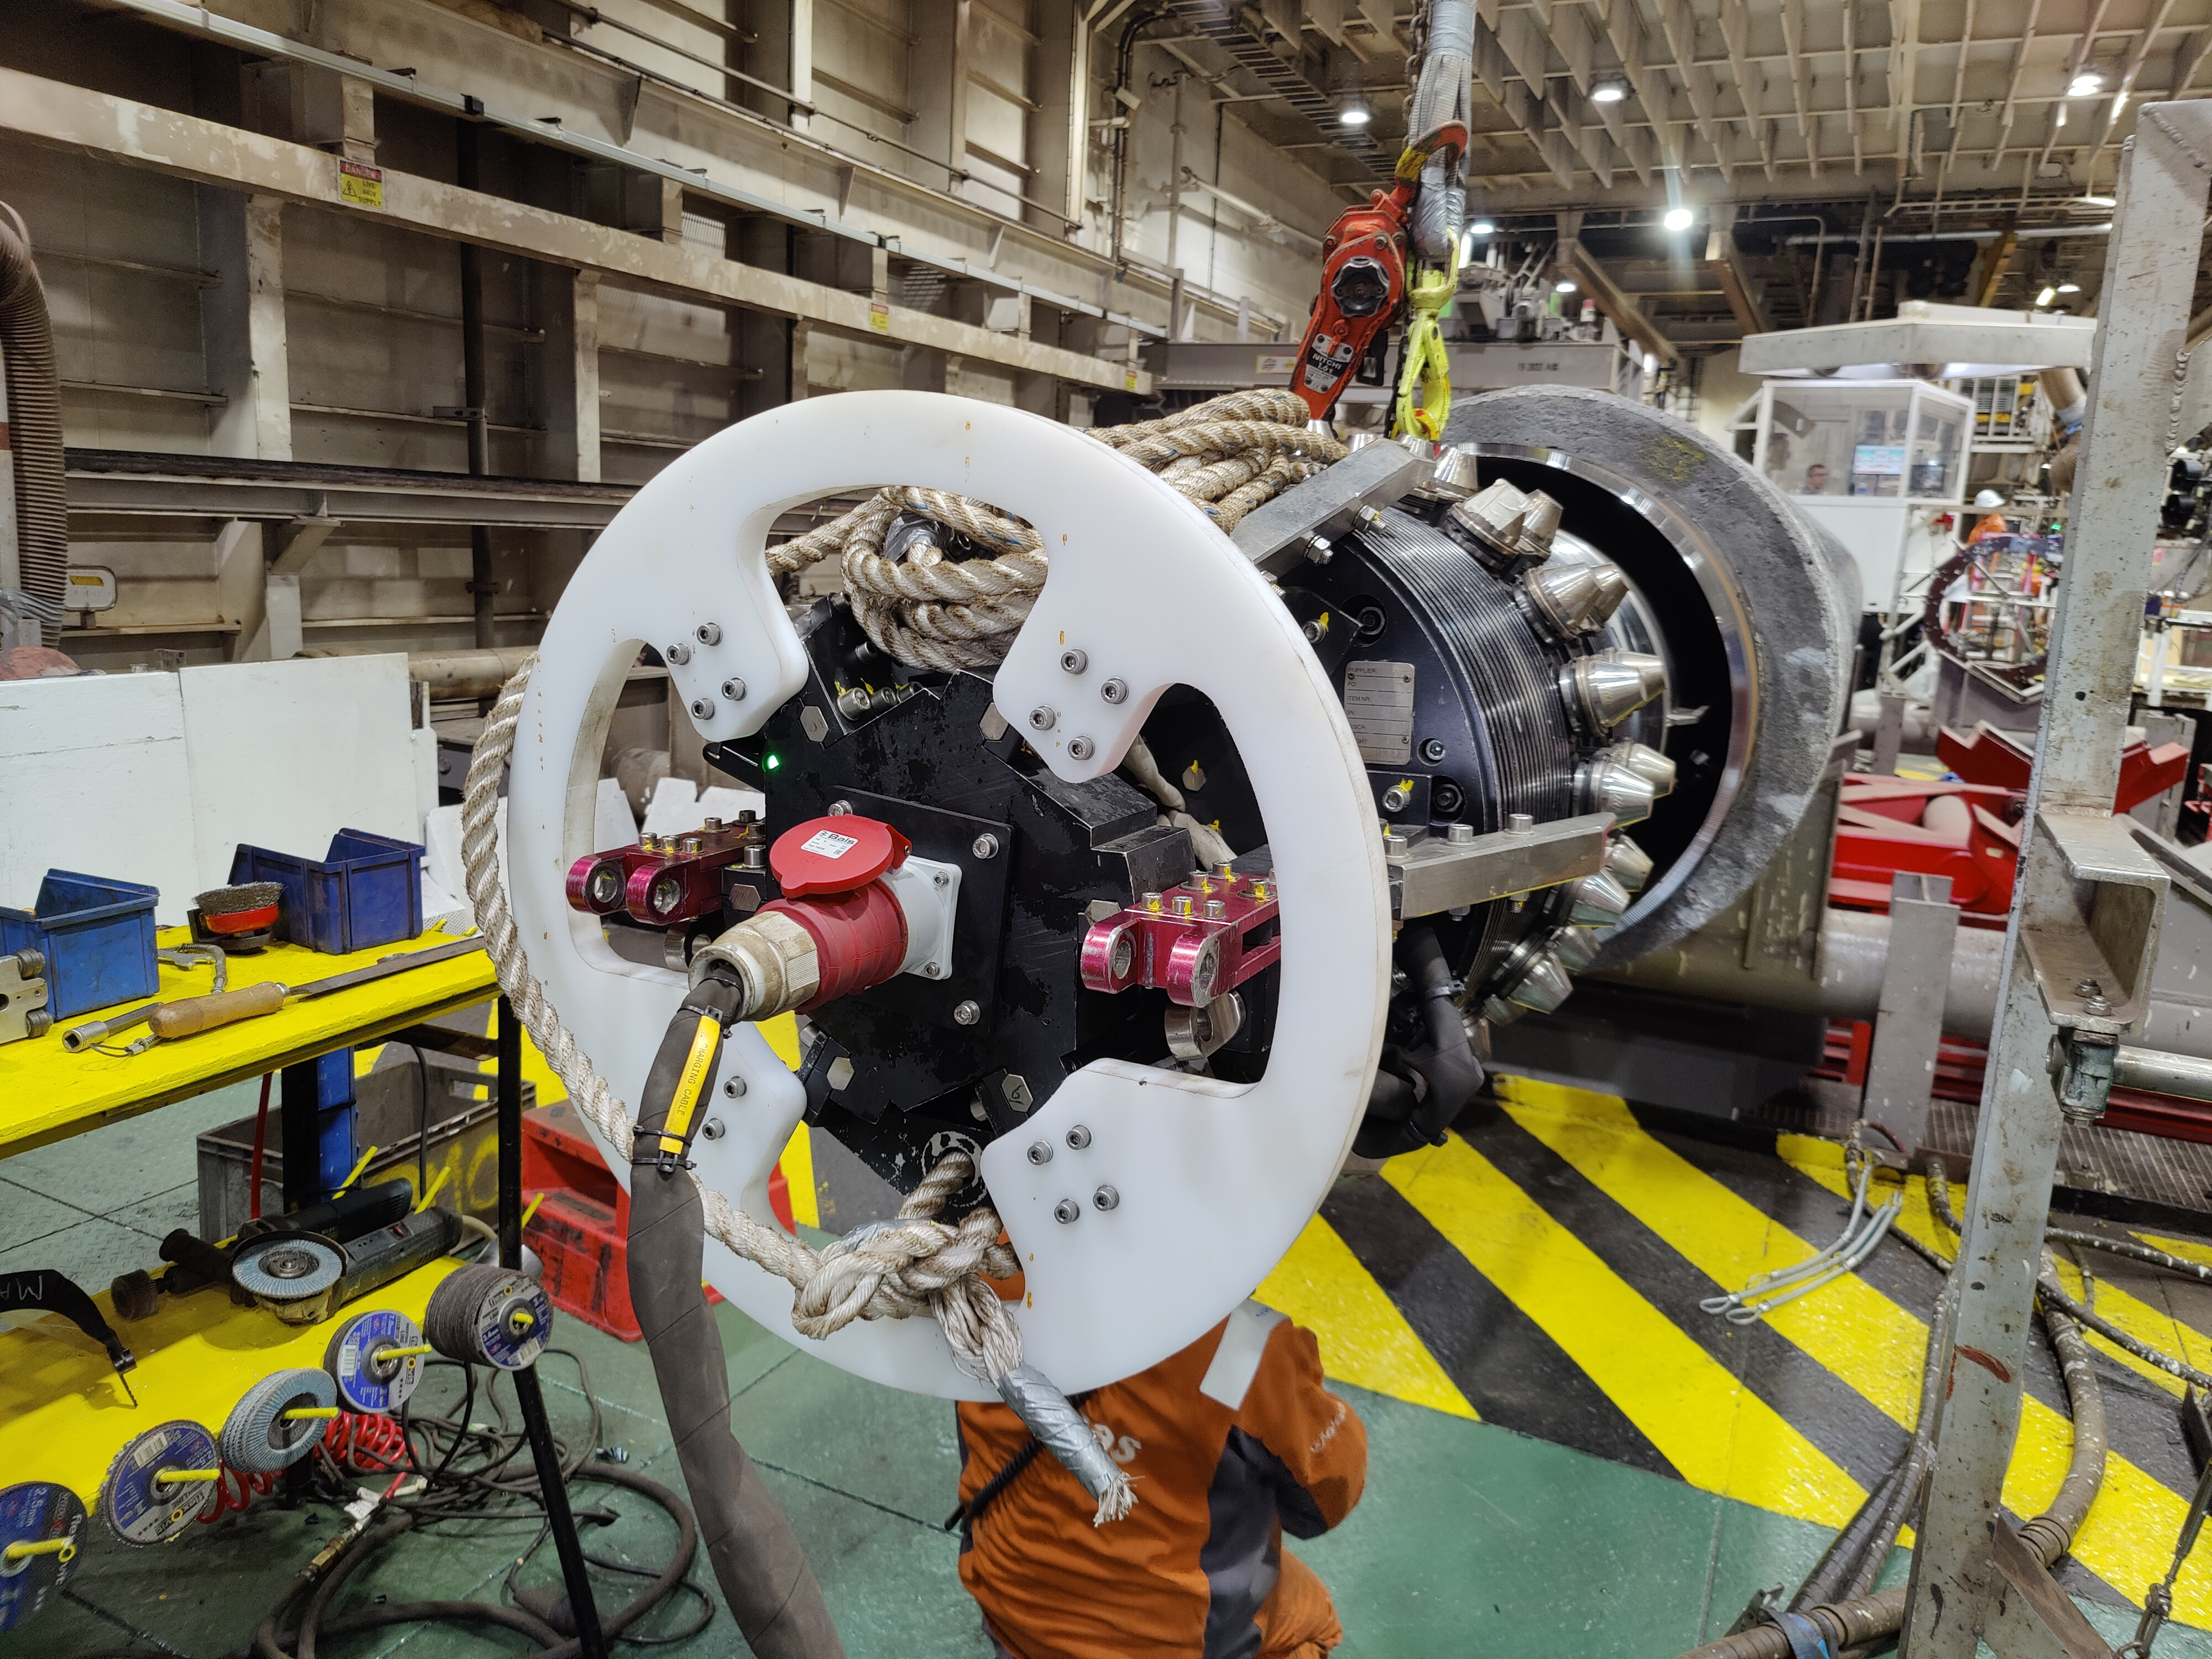
\includegraphics[width=0.7\textwidth]{images/ILUC.jpg}
    \caption{The Internal Line Up Clamp (ILUC). The ILUC sits in the main line, while the new join is shifted over it during line up.
        Its purpose is to steady the main line and new joint pipe ends after line up and during welding. Using a set of pneumatic knobs
        portruding from its exterior it pushes both pipe ends outward, ensuring a circular fit.
        Part of the ILUC is a black ribbed cylinder.}
    \label{fig:iluc}
\end{figure}

Recognising the ILUC gives a good indication of where the main line
is before it can be measured, seeing as the U-Frame passes over the ILUC before it reaches the main line.
Early estimation of the positon and orientation of the main line benefits the overall speed of the process,
because less corrections have to be made in the final line up stage.

Therefore, the final step of the internship is the development of a new part of the recognition software finds the a specific part of
the ILUC; its ribbed cylinder. As before, accuracy and reliability can be tested using the test set-up in the yard. Furthermore,
a combination of different kinds of line, plane and circle fitting algorithms based on minimization of geometric distances can
be used for this. Lastly, Where pipe ends tend to have deformations due to manufacturing, pre-heating or bevelling,
the ILUC is a near-perfect cylinder with a defined radius. This can be used to improve the accuracy of the fitting algorithms.
\begin{flushright}
    $\rightarrow$ internship goal \ref{ssec:intern_goals} \textbf{c}
\end{flushright}